\section{Part 2: Configuration of Flow sheet and Trend}

In this part we got to know the basic functions and menus. We also added the motor control module, which at first was tested in internal mode by hooking the "Start" output to the "kontaktor", and sending a running signal back. To make the motor start, we needed to connect the Motor/Start in RMP422.

To implement the logic control, we read a lot on "additional information" on the motor control module, and decided to use the following terminals:

NotOk1 = 1, Motor stopped if it is running and restart is blocked.

NotOk1 = 0, Start possible if external mode is activated and Off is connected.

InEx = 1, External mode.

InEx = 0, Internal mode.

Off = 0, OnOff enabled.

Off = 1, OnOff disabled.

OnOff = 0, initial value.

OnOff = 1, starts the motor if following criterias is forfilled: 

\textbf{InEx = 1, Off is connected, NotOk1 = 0.}\\

\newpage
We then implemented two "plclg" modules, where the first one triggered the NotOk1 terminal by having: Auto.invMeas \textbf{AND} 0or1.invMeas. This logic implies that the motor will always (hence logic) go to "safe-state" when switching to \textbf{mode 0}, stopping the motor if it is running and block restart.

The second "plglg" were used to implement the logic for external start. To do this, we used the RS block (Set-Reset), so that we were able to set the OnOff terminal by switching Start at the switch, and also reset the RS block when losing 0or1 high. This creates some form of redundancy in the system, having two logic functions stopping the motor if the switch turns to position 0.

We did not use the terminal NoILock1, which is a terminal that overrides the NotOk1 terminal, to improve the safety complexity. The \textbf{InEx} was connected to Auto.invMeas, making internal start impossible when the switch is not in Auto.

\begin{figure}[!htb]
    \centering
    \centerline{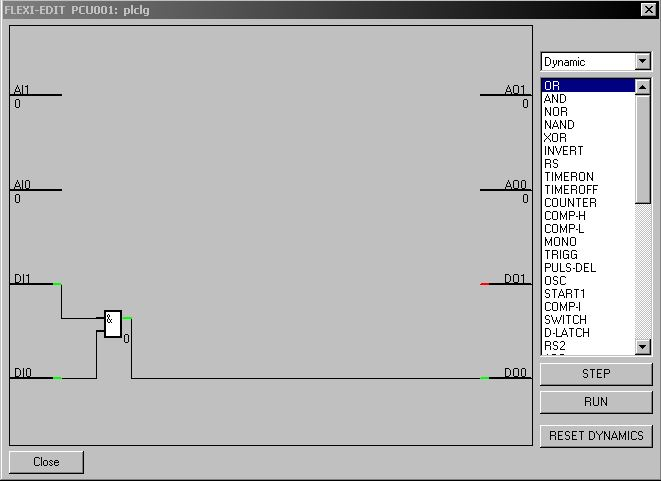
\includegraphics[width=1.1\textwidth]{images/bilde3}}
    \caption{plclg 1}
    \end{figure}
    
\begin{figure}[!htb]
    \centering
    \centerline{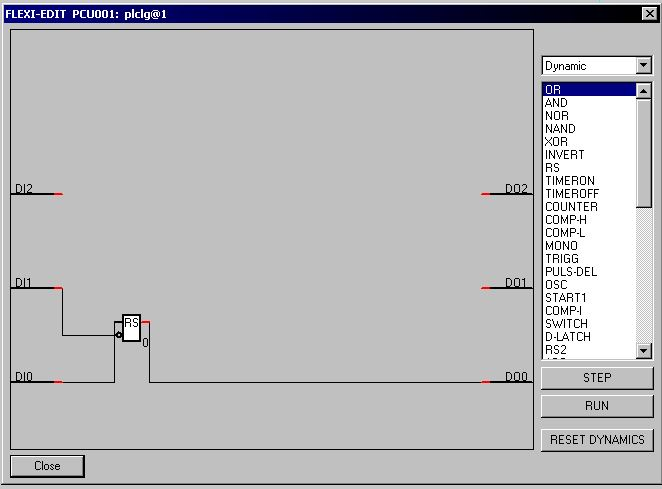
\includegraphics[width=1.5\textwidth]{images/bilde2}}
    \caption{plclg 2}
    \end{figure}

\newpage
Testing our logic, it turned out very well, functioning as described in the assignment text. 
    
Improving our logic, we could have made everything in one plclg module, with \textbf{4 DI} terminals and \textbf{2 DO} terminals.

\begin{figure}[t]
    \centering
    \centerline{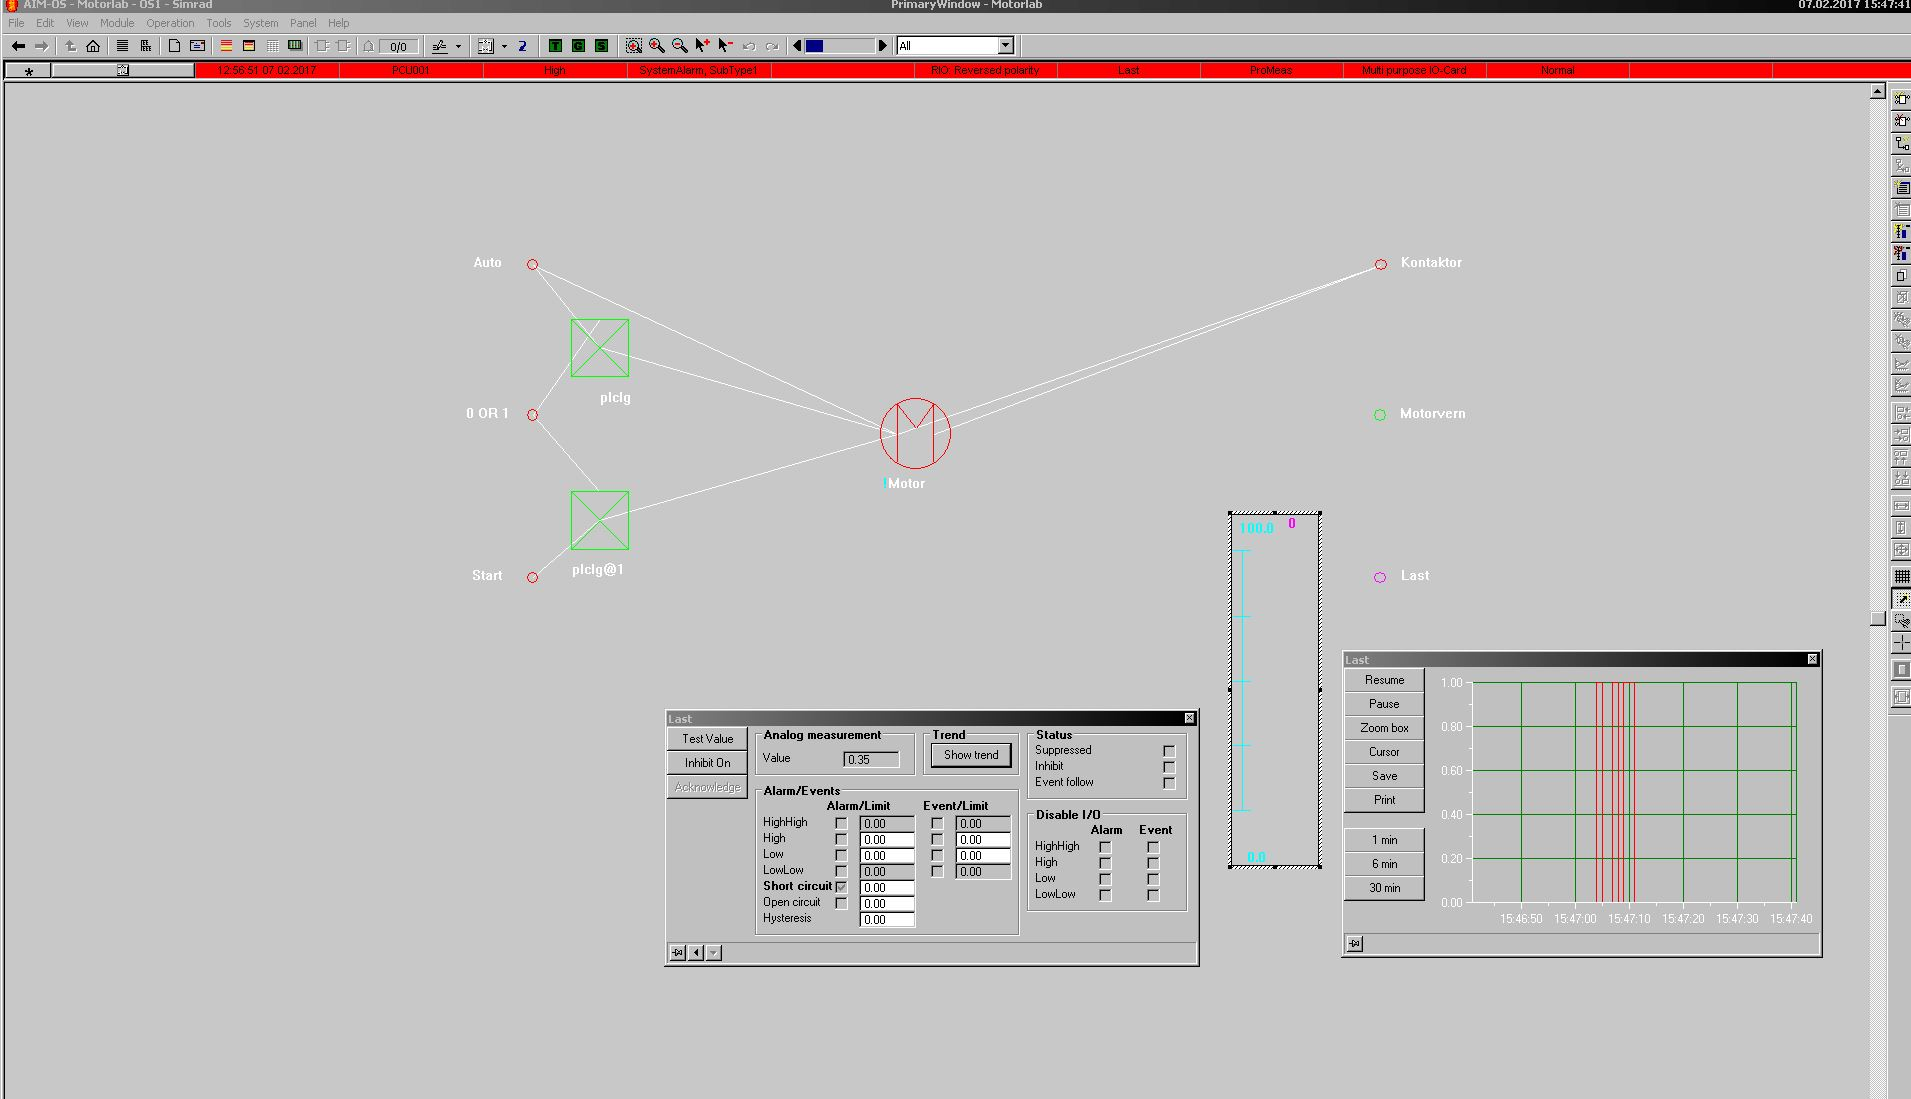
\includegraphics[width=1.5\textwidth]{images/bilde1}}
    \caption{System Overview}
    \end{figure}
\newpage
When the motor logic functioned as desired, it was time to implement a measurement module for the load. This was done using a bar graph, ranging from 0 to 100. To do this we first created an Alarm. 

Scaling the measurement signal in the Parameter View window, was harder than we thought. It seemed like the bias functioned as some kind of off-set, and the gain as some king of multiplier for the signal. Setting these parameters to gain = 5 and bias = 1.3 made the bar graph represent the load ranged from 0-400 as $0-100\%$, triggering the motor protecting when the load closed up on $100\%$.

We also created a time-series for the load, with historical storage ENABLED.
\newpage
\textbf{Creating Trend:}

New image created, where a new curve was defined under the name Last/Meas1/PRIM.

Due to the timeseries, we could move in/out of the trend-image. If this was deactivated, the trend would always start from the beginning.

\begin{figure}[!htb]
    \centering
    \centerline{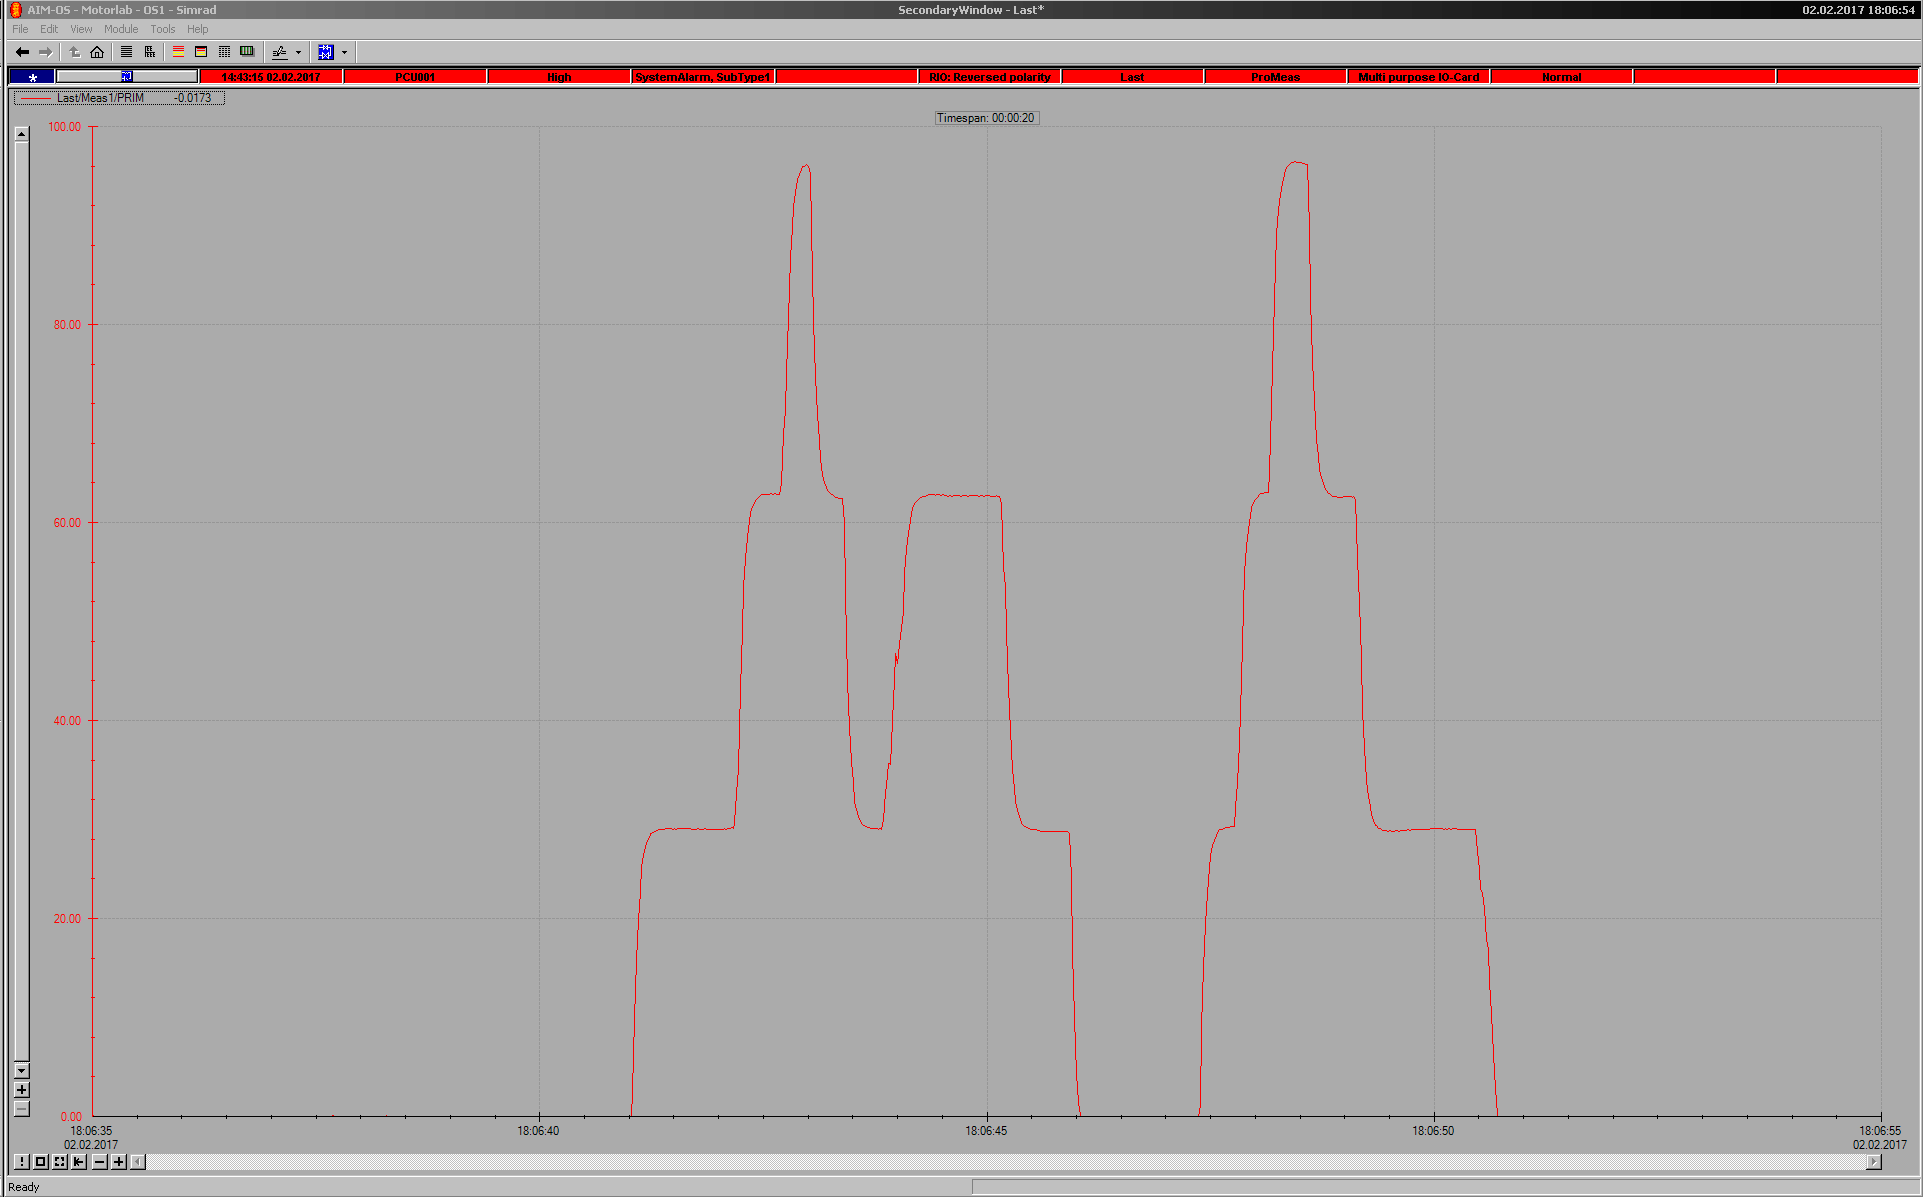
\includegraphics[width=1.5\textwidth]{images/Trend}}
    \caption{Trend Image}
    \end{figure}
    

\newpage
\textbf{Alarms:}

We created the alarms shown below. One for the load exceeding 100 (low priority, yellow), one for the switch not being in Auto (low priority, yellow) and one for the motor protection (high priority, red).

\begin{figure}[!htb]
    \centering
    \centerline{
\includegraphics[width=1.5\textwidth]{images/alarm1}}
    \caption{Load Alarm}
    \end{figure}
    

\begin{figure}[!htb]
    \centering
    \centerline{
\includegraphics[width=1.5\textwidth]{images/Alarm2}}
    \caption{Not in Auto Alarm}
    \end{figure}
    

\begin{figure}[!htb]
    \centering
    \centerline{
\includegraphics[width=1.5\textwidth]{images/Alarm3}}
    \caption{Alarm for Motor Protection}
    \end{figure}









